\documentclass{standalone}
\usepackage{tikz}
\begin{document}

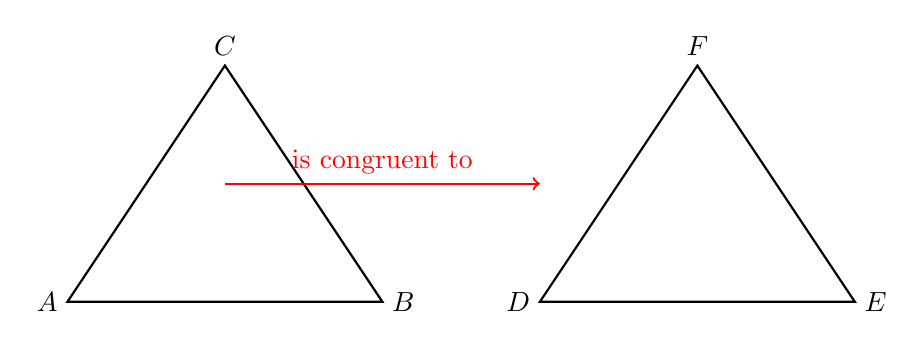
\begin{tikzpicture}

% Define points for triangle ABC
\coordinate [label=left:$A$] (A) at (0,0);
\coordinate [label=right:$B$] (B) at (4,0);
\coordinate [label=above:$C$] (C) at (2,3);

% Draw triangle ABC
\draw [thick] (A) -- (B) -- (C) -- cycle;

% Define points for triangle DEF
\coordinate [label=left:$D$] (D) at (6,0);
\coordinate [label=right:$E$] (E) at (10,0);
\coordinate [label=above:$F$] (F) at (8,3);

% Draw triangle DEF
\draw [thick] (D) -- (E) -- (F) -- cycle;

% Draw red arrow
\draw[->, red, thick] (2,1.5) -- (6,1.5);

% Add text above the arrow
\node[above] at (4,1.5) {\textcolor{red}{is congruent to}};

\end{tikzpicture}

\end{document}
